%
% The first command in your LaTeX source must be the \documentclass command.
\documentclass[sigconf]{acmart}
\settopmatter{printacmref=false} % Removes citation information below abstract
\renewcommand\footnotetextcopyrightpermission[1]{} % removes footnote with conference information in first column
\pagestyle{plain}
\setcopyright{none}
\def\BibTeX{{\rm B\kern-.05em{\sc i\kern-.025em b}\kern-.08emT\kern-.1667em\lower.7ex\hbox{E}\kern-.125emX}}
\newcommand{\opinion}[5]{$$\omega_{#1} = (#2, #3, #4, #5)$$}
\usepackage{mathbbol}
\begin{document}

%
% The "title" command has an optional parameter, allowing the author to define a "short title" to be used in page headers.
\title{COMP 8920 - Section 02: Computational Reasoning in AI\\ Research Essay \\ Argumentation and Subjective Logic}


\author{Vijay Rajasekar Thirulokachander}
\affiliation{%
  \institution{University of Windsor}
  \country{105092311}}
\email{thirulo@uwindsor.ca}

%
% By default, the full list of authors will be used in the page headers. Often, this list is too long, and will overlap
% other information printed in the page headers. This command allows the author to define a more concise list
% of authors' names for this purpose.
\renewcommand{\shortauthors}{Vijay Rajasekar Thirulokachander}

%
% The abstract is a short summary of the work to be presented in the article.
\begin{abstract}
This essay seeks to highlight the advances made in the domain of argumentation theory in artificial intelligence and subjective logic. This involves an analysis of how argumentation is handled in AI, the problems in its implementation, and how research in the application of Subjective Logic in argumentation can help address these problems. We also take a look at the practical implementation of argumentation and subjective logic to understand their potential in different fields of discourse.
\end{abstract}

%
% The code below is generated by the tool at http://dl.acm.org/ccs.cfm.
% Please copy and paste the code instead of the example below.
%
\begin{CCSXML}
  <ccs2012>
  <concept>
  <concept_id>10003752.10003790.10003794</concept_id>
  <concept_desc>Theory of computation~Automated reasoning</concept_desc>
  <concept_significance>500</concept_significance>
  </concept>
  <concept>
  <concept_id>10010147.10010178.10010187.10010190</concept_id>
  <concept_desc>Computing methodologies~Probabilistic reasoning</concept_desc>
  <concept_significance>500</concept_significance>
  </concept>
  <concept>
  <concept_id>10010147.10010178.10010187.10010198</concept_id>
  <concept_desc>Computing methodologies~Reasoning about belief and knowledge</concept_desc>
  <concept_significance>500</concept_significance>
  </concept>
  </ccs2012>
\end{CCSXML}
\ccsdesc[500]{Theory of computation~Automated reasoning}
\ccsdesc[500]{Computing methodologies~Probabilistic reasoning}
\ccsdesc[500]{Computing methodologies~Reasoning about belief and knowledge}

%
% Keywords. The author(s) should pick words that accurately describe the work being
% presented. Separate the keywords with commas.
\keywords{argumentation, reasoning, subjective logic}


%
% This command processes the author and affiliation and title information and builds
% the first part of the formatted document.
\maketitle

\section{Introduction to Argumentation Theory}
Douglas Walton, in the book \textit{Argumentation in Artificial Intelligence }\cite{rahwan2009argumentation}, defines an \textit{argument} as a set of statements made up of three parts: a conclusion, a set of premises and an inference from the premises to the conclusion. Furthermore, an argument can be supported by other arguments, or it can be attacked by other arguments, and by raising critical questions about it.

In the \textit{Handbook of Argumentation Theory}, van Eemeren et al. describe the term \textit{Argumentation} as below:

\begin{quote}Argumentation is a communicative and interactional act complex aimed at resolving a difference of opinion with the addressee by putting forward a constellation of propositions the arguer can be held accountable for to make the standpoint at issue acceptable to a rational judge who judges reasonably.\cite{book:1206719}\end{quote}

\textit{Argumentation Theory} is the study of argumentation in all its manifestations and varieties, regardless of the angle at which it is approached, the primary research interest with which it is studied and the background of the theorists who study it. The scope of argumentation theory is very broad. It ranges from argumentation in public and professional settings, as well as personal settings. Argumentation theory deals with factors playing a part in resolving differences of opinion by means of argumentative discourse for which the participants can be held responsible.\cite{book:1206719}

There are four tasks undertaken by argumentation, viz. \textit{identification, analysis, evaluation and invention}\cite{rahwan2009argumentation}: 

\begin{itemize}
  \item \textbf{Identification}: To identify the premises and conclusion of an argument as found in a text of discourse. A part of this task is to determine whether a given argument found in a text fits a known form of argument called an argumentation scheme. 

  \item \textbf{Analysis}: To find implicit premises or conclusions in an argument that need to be made explicit in order to properly evaluate the argument. Arguments present in natural language texts of discourse tend to leave premises or conclusions implicit. An argument containing such missing assumptions is traditionally called an enthymeme. 
  
  \item \textbf{Evaluation}: to determine whether an argument is weak or strong by general criteria that can be applied to it.

  \item \textbf{Invention}: To construct new arguments that can be used to prove a specific conclusion.
\end{itemize}

The general approach or methodology of argumentation can be described as distinctively different from the traditional approach based on deductive logic. The traditional approach concentrated on a single inference, where the premises and conclusion are designated in advance, and applying formal logic to determine whether the conclusion conclusively follows from the premises. This approach is often called monological.

In contrast, the argumentation approach is called dialogical (or dialectical) in that it looks at two sides of an argument, the pro and the contra. According to this approach, the method of evaluation is to examine how the strongest arguments for and against a particular proposition at issue interact with each other, and in particular how each argument is subject to probing critical questioning that reveals doubts about it. By this dialog process of pitting the one argument against the other, the weaknesses in each argument are revealed, and it is shown which of the two arguments is the stronger.\cite{rahwan2009argumentation}

A simple way to represent a sequence of argumentation in the dialogical style is to let the nodes in a graph represent arguments and the arrows represent attacks on arguments. An example of such a representation is depicted in Figure \ref{DungArgRep}.

This method of representation of arguments paved the way for research in argumentation in artificial intelligence. This is detailed in the next section of the essay.

\begin{figure}
  \centering
  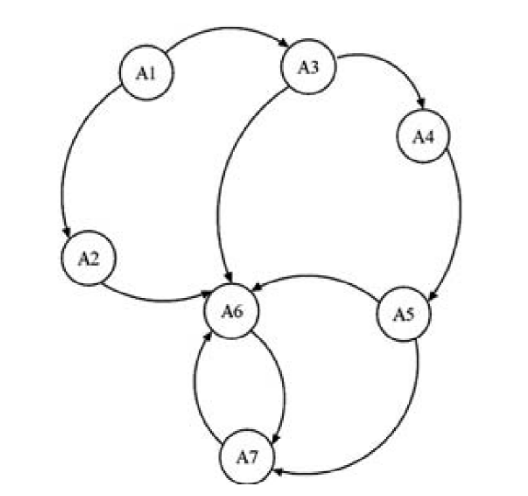
\includegraphics[width=3in]{images/pmdungaaf.png}
  \caption{Dung Argument Representation \cite{rahwan2009argumentation}}
  \label{DungArgRep}
\end{figure}

\section{Argumentation in Artificial Intelligence}
Formal models of argumentation have made significant contributions to Artificial Intelligence, from defining semantics of logic programs, to implementing persuasive medical diagnostic systems, to studying negotiation dialogues in multi-agent systems. On the other hand, Artificial Intelligence has also made an impact on Argumentation Theory and Practice, for example by providing formal tools for argument analysis, evaluation, and visualisation.

Initially, argumentation was implemented as a possible supporting approach to achieve a formal treatment of non-monotonic reasoning, rather than as an independent domain. (A non-monotonic logic is one where conclusions are not final and can be updated when more arguments are provided). The engagement of philosophers and legal theorists with reasoning and argumentation in AI marked a key stage in the move towards computationally grounded models of argument.\cite{BENCHCAPON2007619}

Rahwan et al. in \cite{rahwan2009argumentation} note the significant contributions to research in the field of argumentation in AI during the late 2000s. As evidence for this observation, they mention the appearance of special issues in leading scientific journals such as Springer, Elsevier, IEEE etc. and various workshops dealing with argumentation in AI in those years.

Argumentation in AI is primarily addressed using two major approaches: Abstract Argumentation and Structured Argumentation.

\subsection{Abstract Argumentation}
Abstract argumentation is formalism that, when employed, can provide important insights into the nature of argumentation. As shown in Fig \ref{DungArgRep}, a situation involving argumentation can be represented by a directed graph. Each node represents an argument, and each arc denotes an attack by one argument on another. Such a graph can then be analysed to determine which arguments are acceptable according to some general criteria. As mentioned in the previous section, this was originally proposed in a paper by P. M. Dung, and it has led to a large number of papers that have explored properties and developments of it.

An abstract argument system or argumentation framework is a pair $ <\mathcal{A}, \mathcal{R}>$ consisting of a set $\mathcal{A}$ whose elements are called arguments and of a binary relation $\mathcal{R}$ on $\mathcal{A}$ called attack relation.

A simple argumentation framework that represents an argument $b$ attacking an argument $a$, given a set of arguments $\{a, b\}$ can be represented as below:

$$
b \rightarrow a
$$

and the corresponding AAF representation is: $<\{a, b\}, \{(b, a)\}>$.

AAFs are primarily concerned with the \textit{justification state of arguments}. An argument is considered to be \textit{justified} if it has some way to survive the attacks it receives, as \textit{not justified} (or rejected) if not.


Dung defines two types of semantics to consider an argument to be justified. A semantic is a formal definition of a method used during the argument evaluation. The first type is Labelling-Based Semantics, which is used to assign simple labels such as \textit{in, out, undecided} to measure the validity of arguments. 

The second type is Extension-based Semantics, defined using the following criteria:
\begin{itemize}
  \item \textbf{Conflict Free}: If an argument $a$ is being attacked by an argument $b$, then a set $\{a, b\}$ should not exist for the AAF to be considered conflict-free.
  \item \textbf{Acceptability}: For an argument $b$ to be considered acceptable, if it attacks an argument $a$ present in a set $S$, it should attack every argument in the set $S$
  \item \textbf{Admissibility}: An argumentation framework is considered to be admissible, if and only if is conflict-free and acceptable.
  \item \textbf{Strong Admissibility}: No argument should be able to attack itself
  \item \textbf{Reinstatement}: If an argument is defending itself against one argument in an extension set of arguments, then it should be able to defend itself against every argument in the extension set.
  \item \textbf{Directionality}: A set of arguments is affected only by its ancestors in the attack relation 
\end{itemize}

Dung's paper on AAFs currently has close to 4000 citations on Google Scholar. A variety of improvements to his approach have been suggested and/or implemented over the years. However, a majority of these are beyond the focus of this essay, so they are not discussed here. The above expressed concepts and defintions provide the basis for the implementation of Subjective Logic into AAFs.

\subsection{Structured Argumentation}
In abstract argumentation, each argument is considered to be atomic. There is no specification of what is an argument or an attack. They are assumed to be given. There is also no internal structure
to an argument. This abstract perspective provides many advantages for studying the nature
of argumentation, but it is not enough for understanding argumentation or for
building tools for supporting or undertaking argumentation.

To achieve a deeper understanding, Structured Argumentation is used, with specifications on how arguments and attacks can be constructed. In Structured Argumentation, an argument and an attack can be defined as below:

\begin{itemize}
  \item \textbf{Argument}: A tuple containing premises and conclusions for the argument. May also contain other information regarding how the conclusion is drawn for the premise.
  \item \textbf{Attack}: A binary relation over arguments denoting when an argument attacks another argument.
\end{itemize}

Structured Argumentation can be divided into two different types, monological and dialogical argumentation. In monological argumentation, a set of arguments and counterarguments are analyzed in order to evaluate them, determine whether they are acceptable and derive conclusions based on them. In dialogical argumentation, the focus is on the relationships between arguments and counterarguments, belief updation, etc. It also takes protocols and argumentation strategies into consideration. \cite{besnard}.

Some approaches to Structured Monological Argumentation are Assumption Based Argumentation, ASPIC+, Defeasible Logic Programming, and Deductive Argumentation. These approaches share a lot of similarities, but also differ heavily in terms of implementation and the school of logic used. P. M. Dung also notes the similarities between his AAFs and ABA frameworks.


\subsection{Multi Agent Argumentation}
The term \textit{Computation} often been understood as numerical calculations or the processing of information. However, nowadays it is viewed as distributed understanding and interaction between intelligent entities. This view has had major implications for the conceptualization, design, engineering and control of software systems, most profoundly expressed in the concept of systems of intelligent software agents, or multi-agent systems. Agents are software entities with control over their own execution; the design of such agents, and of multi-agent systems of them, presents major research and software engineering challenges to computer scientists.\cite{rahwan2009argumentation}


Multi Agent Argumentation has been popularly implemented using Dialogue Game frameworks. This involves emulating human dialogue, i.e natural language discourse. A set of semantics, syntaxes, and truthfulness protocols are employed as a formalism derived from human linguistics.
\section{Problems with the Application of Argumentation in AI}
\subsection{Handling uncertainty}
Many frameworks for argumentation ignore probabilistic and
possibilistic concepts, focusing instead purely on the interactions (such as rebutting and undercutting attacks) between arguments. Applying frameworks like these to domains in which uncertain evidence exists is difficult. There is a need for a formalism to represent uncertainty from sources, or uncertainty between arguments and attacks.

\subsection{Enthymemes}
An enthymeme is an argument containing a premise or
conclusion that was not explicitly stated but that is required to make sense of the
argument. For example, if I were to argue, ‘ In some cases, it can be very difficult to fairly judge what the implicit assumption of a given argument is supposed to be

Douglas Walton provides an example for such an enthymeme in \cite{walton2005argumentation}: All philosophers are wise, therefore Confucius is wise’. 

The implicit premise of this argument is the proposition, ‘Confucius is a philosopher’. But this proposition was not stated anywhere, or is not part of an agent's knowledge.
\subsection{Inconsistencies from multiple sources}

One of the principal challenges in a Multi Agent Argumentation system is to make sense of conflicting information. Whether this is a crowdsourcing system where many
contributors send conflicting information, or an application where different sensors
send different information, these systems have to make a decision on what information is truthful, based on a limited model to provide sufficient evidence for the information. This highlights the need for an intelligent agent having to revise its beliefs upon receiving new information.


Belief revision is the process of changing beliefs to adapt the current state of an agent to a new piece of information.\cite{rahwan2009argumentation}. Benferhat et al. in \cite{benferhat1995infer} suggest that in the case of multiple sources of information, revision always comes down to destroying part of the knowledge and it is not necessary to restore consistency in order to make sensible inferences from an inconsistent knowledge base. The argumentation inference can derive conclusions with reasons to believe them. 
\subsection{Representing Accrual of Arguments}
An important concept in argumentation is that the more arguments supporting a conclusion, each of the arguments and the conclusion become stronger themselve. However, as more arguments begin to accrue, there are certain issues with this process. These issues that were identified by Prakken in \cite{Prakken:2005:SAA:1165485.1165500} are listed as follows:
\begin{itemize}
  \item Accruals are sometimes weaker than their elements.
  \item An accrual makes its elements inapplicable.
  \item Flawed reasons or arguments may not accrue.
\end{itemize}
Before we take a look at how these problems are approached through the use of Subjective Logic, let us first describe Subjective Logic in the next section.
\section{A Short Introduction to Subjective Logic}
In binary logic a proposition about the state of the world must be either true or
false, which fits well with an assumed objective world. Probability calculus takes
argument probabilities in the range [0,1], and hence to some extent reflects subjectivity by allowing propositions to be partially true. However, we are often unable to estimate probabilities with confidence because we lack the necessary evidence. A
formalism for expressing degrees of uncertainty about beliefs is therefore needed in
order to more faithfully reflect the perceived world in which we are all immersed.
In addition, whenever a belief about a proposition is expressed, it is always done by
an individual, and it can never be considered to represent a general and objective
belief. It is therefore necessary that the formalism also includes belief ownership in
order to reflect the fundamental subjectivity of all beliefs.\cite{josang2016subjective}

In subjective logic, we can represent an opinion as \opinion{x}{b_x}{d_x}{u_x}{a_x} where $b_x$ represents belief mass distribution, $d_x$ represents disbelief, $u_x$ represents uncertainty mass and $a_x$ represents base rate. 

This opinion representation can be visualized as a barycentric system with three axes, forming a triangle. One vertex represents a belief value of 1 and disbelief value of 0, another vertex representing a disbelief value of 1 and belief value of 0, and the third vertex representing an uncertainty value of 1. An example of this representation is depicted in Fig \ref{barycentric}

\begin{figure}
  \centering
  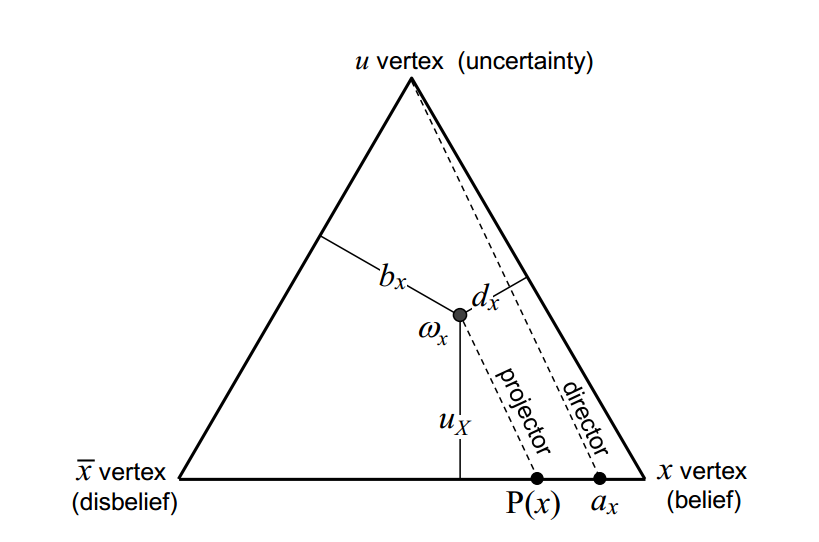
\includegraphics[width=3in]{images/barycentric.png}
  \caption{Barycentric Opinion Representation \cite{josang2016subjective}}
  \label{barycentric}
\end{figure}

The advantages of using subjective logic are that real-world situations can be
realistically modelled with regard to how those situations are perceived, and that conclusions more correctly reflect the ignorance and uncertainties that necessarily result from partially uncertain input arguments. Subjective logic has the advantage of providing advanced operators for Dirichlet PDFs, for which no practical analytical solutions previously existed. It should be mentioned that the simplicity of some SL operators comes at the cost of allowing those operators to be approximations of the analytically correct operators. 


\section{Subjective Logic in Argumentation}
The earliest work implementing Subjective Logic in Argumentation was published in 2007 by Oren et al. in their paper \textbf{\textit{Argumentation Based Contract Monitoring in Uncertain Domains}}. The authors provide a new framework that uses Subjective Logic concepts to represent uncertainty in an argumentation environment. 

In the same year, they published another paper titled \textbf{\textit{Subjective logic and arguing with evidence}}, which sought to improve existing argumentation frameworks by taking important factors such as accrual of arguments, argument schemes and burden of proof into consideration when constructing a framework.

Oren's final work in 2007 implementing Subjective Logic in Argumentation was \textbf{\textit{An Argumentation Framework Supporting
Evidential Reasoning with Applications to Contract Monitoring}}. He claimed that his research proposed both abstract and concrete models addressing the problem of how toargue with evidence. He also claimed that unlike other work, their approach advanced a unified model, dealing with issues arising at the logical, dialectic, procedural and heuristic levels\cite{oren2007argumentation}.

There was not much research taking place in this fairly new domain for the next 10 years. In 2016, Koster et al. published a paper titled \textbf{\textit{Liar liar, pants on fire; or how to use subjective logic and argumentation to
evaluate information from untrustworthy sources}}. As the title suggests, the authors came up with a new type of operator named Belief Revision Operator to update beliefs while addresssing uncertainty in an environment and implemented a preference-based argumentation framework along with trust models and subjective logic. This paper was cited by Prof. Josang's paper on the topic of argumentation in subjective logic\cite{8455455}. 

In 2017, duy Hung published a paper \cite{8023355} expressing a method to combine Dempster Shafer belief theory with Assumption Based Framework built on top of Probabilistic Logic. Even though this paper did not use Subjective Logic proposed by Prof. Josang, the author still compared his use of DST with SL as the latter is derived from the former.

In 2018, Prof. Josang published his approach towards the use of Subjective Logic in Argumentation. This approach was primarily targeted at handling fallacies or enthymemes in arguments present in an AAF. To achieve this, they come up with a new type of AAF named slAAF, where arguments can have belief and disbelief values.

There have been very few papers implementing the concepts of Subjective Logic in argumentation. However, given the broad scope of Argumentation as a field, there is a possibility that more research will be published in the near future tackling the problems present in argumentation using SL.

Let us see how the abovementioned papers address the problems mentioned in Section 4 of this essay.

\subsection{Handling Accrual of Arguments}
Oren et al. \cite{OREN2007838} attempt to address situations consisting of different agents that are trying to reach a shared conclusion about a particular state of the environment 
they are present in. Various assumptions are made, such as: 
\begin{itemize}
  \item the information obtained through sensors could potentially be wrong, 
  \item some subsets of the environment are observable
  \item agents are self interested and may have opposing goals 
\end{itemize}

The authors point out the weaknesses in the probabilstic approaches concerning the construction of evidence based argumentation frameworks as they perform 
inference when faced with uncertainty and conflicting arguments. They identified the need for four layers of an argument framework to have agents engage in dialogue 
and obtain shared information from different sensors to construct a shared world view. These layers are implemented as below:
\begin{itemize}
  \item Logical Layer: Built using Subjective Logic as proposed by Prof. Josang
  \item Dialectic Layer: Construction of arguments and represent the accrual of arguments and argument schemes
  \item Procedural Layer: Sensors to capture environment information
  \item Heuristic Layer: Provides decision making capabilities for the agents to decide on which sensors to use for probing
\end{itemize}

Across multiple layers of the framework, instances of arguments are represented in the form 
of tuples comprised of a set of Possible Facts about the universe associated with the environment and a set of Argument Schemes.
An example consisting of two agents and a set of argument schemes is set up with the intent to determine the amount of building materials required. Agent $\alpha$ is 
assigned to be responsible for the stock and supply of steel, whereas $\beta$ is responsible for the supply of concrete. Both agents have self-serving (opposing) 
agendas in the same environment - to minimize the amount of their corresponding building material used in the bridge.

A set of argument schemes consisting of the various requirements that each material must satisfy for its use is defined. On experimentation, a dialogue takes place 
between the two agents by each probing a different sensor of the other to see if the building conditions are satisfied in a manner most suitable to its 
own goal. To tackle uncertainty of any sensor, belief opinions are used. As the dialogue proceeds, each agent accrues a set of arguments that assign an opinion 
value to its base predicates.

The authors observed that both agents agreed to come to a solution that satisfies their self serving goals. Through repeated probing of sensors and 
handling of uncertainty, arguments were accrued in favor of one agent. Fig. \ref{fig:fig1} represents the dialog that took place between the two agents and the probing of various sensors.

\begin{figure}
  \centering
  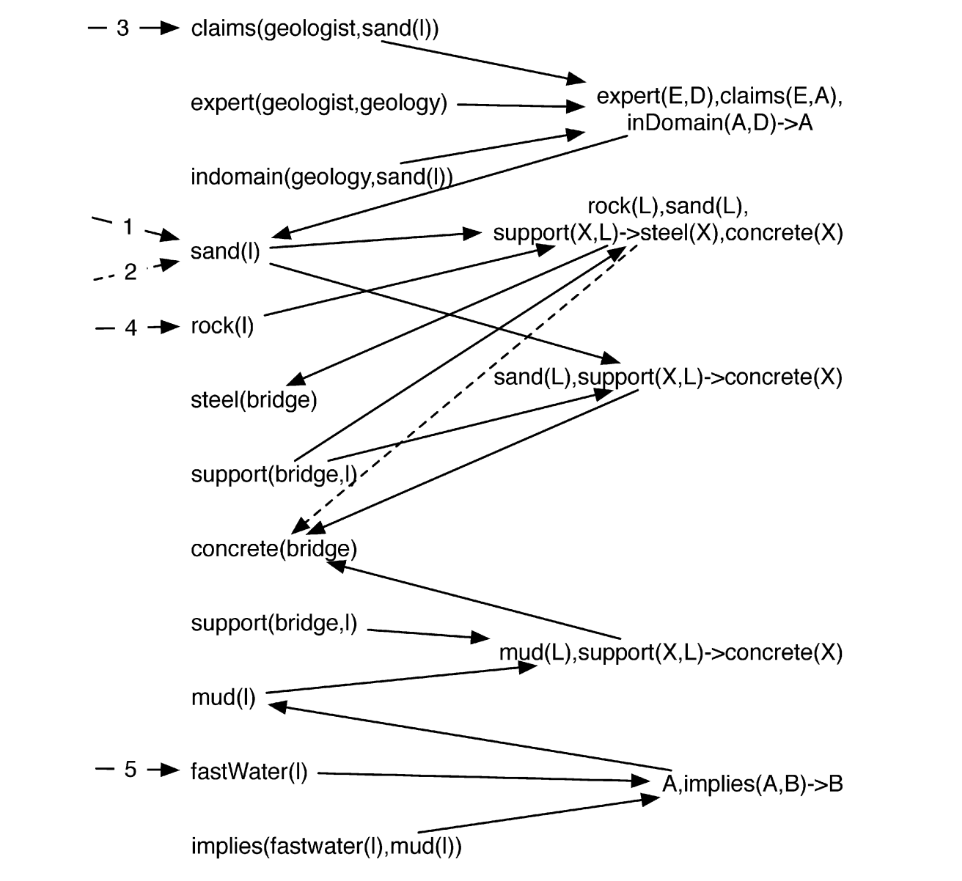
\includegraphics[width=3in]{images/dialog.png}
  \caption{Dialog Argument Graph between the two agents. Image taken from \cite{OREN2007838}.}
  \label{fig:fig1}
\end{figure}

The authors claim that the model is general enough to be applied to almost any area in which argument is employable. However they also state that 
this applies only to the lower levels of the model, whereas the higher levels require evidence based reasoning. In the future, they aimed to enrich the sensor model 
in order to provide better opinions on information as well as to achieve a mapping between dialogue based argument framework and Dung's argumentation Framework \cite{DUNG1995321}.
\subsection{Josang's slAAFs}
In 2018, Santini et al. published their approach towards handling enthymemes and uncertainty in P. M. Dung's Abstract Argumentation Frameworks. To achieve this, they improve upon a Constellations approach defined in \cite{dung2010towards} that assigns a probability distribution over argument sets.  They replaced the probability distribution with Subjective Logic since SL provides a mechanism to take uncertainty into account. An AAF that
uses Subjective Logic is defined by the authors to be an slAAF. The paper measures the impact of subjective opinion on the parameters required for an argument to be considered an \textit{Accepted Argument} viz. conflict-free sets, admissible sets, complete semantics, preferred semantics and stable semantics. An AAF consisting of arguments that can be considered Accepted Arguments can be induced from an slAAF if it satisfies the 
following criteria:
\begin{itemize}
  \item The set of arguments in the AAF is a subset of the arguments in the slAAF,
  \item The attacks in the AAF are a subset of the intersection of the set of attacks in the slAAF with the Cartesian product of the set of induced arguments with itself,
  \item For every argument in the set of arguments in the slAAF, the belief score is 1.
  \item For every attack between two arguments in the slAAF, the belief score is 1.
\end{itemize}
In the induced AAF, the set of arguments consisting of enthymemes and fallacies are assigned a belief score of lower than 1 and an uncertainty score greater than 1. The sum of all expectation values of all the AAFs that can be induced from an slAAF is 1.

The authors also analyse different approaches towards fusion of subjective belief in the Constellations approach. \textit{Averaging Fusion} is used for fusing beliefs over a set of 
arguments in an slAAF.

\subsection{Using SL to evaluate information from untrustworthy sources}
Koster et al., in \cite{Koster2017} approach the conflict of arguments and information in a system where communication between agents plays
a major role in the functioning of the system. The system has to decide which agent is providing more trustworthy information
and the revision of belief based on trustworthiness. 

To achieve this, the authors propose a new type of Belief Change Operator. The agent receives information in two forms: large amount of conflicting data, and a belief change operator that includes subjective logic
into an argumentation framework to make the agent provide higher importance to some part of the conflicting data over the rest. They use 
the argumentation framework suggested by Amgoud and Vesic in \cite{AMGOUD2014585} as they believe it provided a better way of representing preference
ordering using subjective logic compared to Dung's \cite{DUNG1995321} AAF model.

The authors also detail a set of specifications that determine how an agent's beliefs are computed based on received information. These are defined as follows:

\begin{enumerate}
  \item Information collection
  
  A trust model is used to determine how trustworthy a source is and how credible the information provided by the source is. The authors claim that 
    most belief revision operators do not focus on this step as much as they do on deciding what information to believe in.

  
  \item Aggregation of Information
  
  To combine the opinion of different opinions of the same proposition, the cumulative fusion operator
  is used.

  \item Selection of Information to believe in
  
  On a set of Arguments that can be generated from a set of Propositions a resulting base belief set is obtained. We provide a 
  preference relation to this set. A tuple consisting of a set of arguments, the relationships between these arguments, and the preference ordering 
  of these arguments acts as the Belief Change Operator.

  
\end{enumerate}
\section{Applications of Argumentation in AI}
Argumentation in AI has found applications in a variety of domains that inherently involve discourse. Tools have also been developed to standardize implementation of argumentation in software development. In this section we will first take a look at some of these applications and tools, followed by a short observation of applications involving SL in argumentation.

\subsection{Law}
As a natural application of argumentation, discourse in law possesses distinctive features:
\begin{itemize}
  \item Any proposed set of rules inevitably contain gaps, conflicts, and loopholes
  \item Many of its concepts are imprecisely defined meaning that interpretation is required
  \item Much legal argumentation is adversarial and dialectic in nature
  \item Conclusions are defeasible, subject often to formal appeal.
\end{itemize}
All of these features mean that deduction cannot provide an adequate model of legal reasoning and instead argumentation must take centre stage to allow for these contextual, procedural and interpretative elements. For this reason developments in computational models of argumentation have been readily taken up by the AI \& Law community. Equally, however, the legal AI community has contributed much to computational models of argumentation: a considerable amount ofthe work described in this book has its origins in work motivated by legal applica-tions, and more than half the chapters have authors who have published in specialist AI \& Law venues. The legal domain thus acts as both a motivation and a test-bed for developments in argumentation in AI.

\subsubsection{TAXMAN} One of the earliest practical applications of Argumentation in law is TAXMAN, a program written in C, to aid tax lawyers in applying taxation to corporate reorganization in the year 1976. McCarty, the creator of this program, claims in \cite{mccarty1976reflections} that TAXMAN is an important tool for the development of theories of legal reasoning. He also claims that it is a powerful alternative to a sequence of preprogrammed questions and answers, and that his work is modelled based on a branch of study known as artificial intelligence.

\subsubsection{Argument Retrieval Systems} Legal discourse involves not just rules and statements, but also the context and supporting arguments that make up a ruling of law. Ashley and Walker in \cite{ashley2013information} describe how advances in text annotation, statistical text analysis, and machine learning, coupled with argument modeling in AI and Law, can support extracting argument related information from legal texts. This could enable systems to retrieve arguments as
well as sentences, to employ retrieved information in proposing new arguments, and to
explain any proposed evidence or conclusions. They are currently researching how a program
could learn to extract this argument-related information from new case texts using a
multi-level annotation approach based on the DeepQA architecture of the IBM Watson
question-answering system.

\subsection{Machine Learning}
Two different papers addressing the use of Argumentation in Machine Learning provide frameworks for the implementation of learning methods using arguments.

The first paper, published by Gomez and Chesnevar in 2004 \cite{defeasibleML}, highlights the features common to most argumentation framework: Knowledge Based Formalization, the definition for an argument, and dialectical reasoning. They identified the possibility that a Machine Learning model can also be developed using the same framework. 

\begin{itemize}
  \item Building a defeasible knowledge base from training data
  \item Building arguments from the knowledge base using a combination of analytical learning methods (explanative learning) and inductive learning methods (neural nets)
  \item Dialectical reasoning by implementing defeasbility using numeric and probabilistic values
\end{itemize}

In 2015, Xu et al. \cite{ensemblelearning} proposed an Ensemble Learning approach to implement 
machine learning using argumentation \textbf{AMAJL}. The model of AMAJL is depicted in Fig \ref{fig:ens}. As shown in the figure, AMAJL consists of three stages: 
\begin{enumerate}
  \item Sampling stage: An individual agent generates its training sample by sampling with replacement from the training data.
  \item Mining stage: Agents perform data mining on respective samples to generate individual knowledge bases
  \item Argumentation stage: For each sample (can be treated as argumentation topic) in training dataset, agents use individual knowledge to perform argumentation on Arena for obtaining an optimal knowledge of this topic, which will be stored in the global knowledge base of ensemble classifier.
\end{enumerate}
\begin{figure}
  \centering
  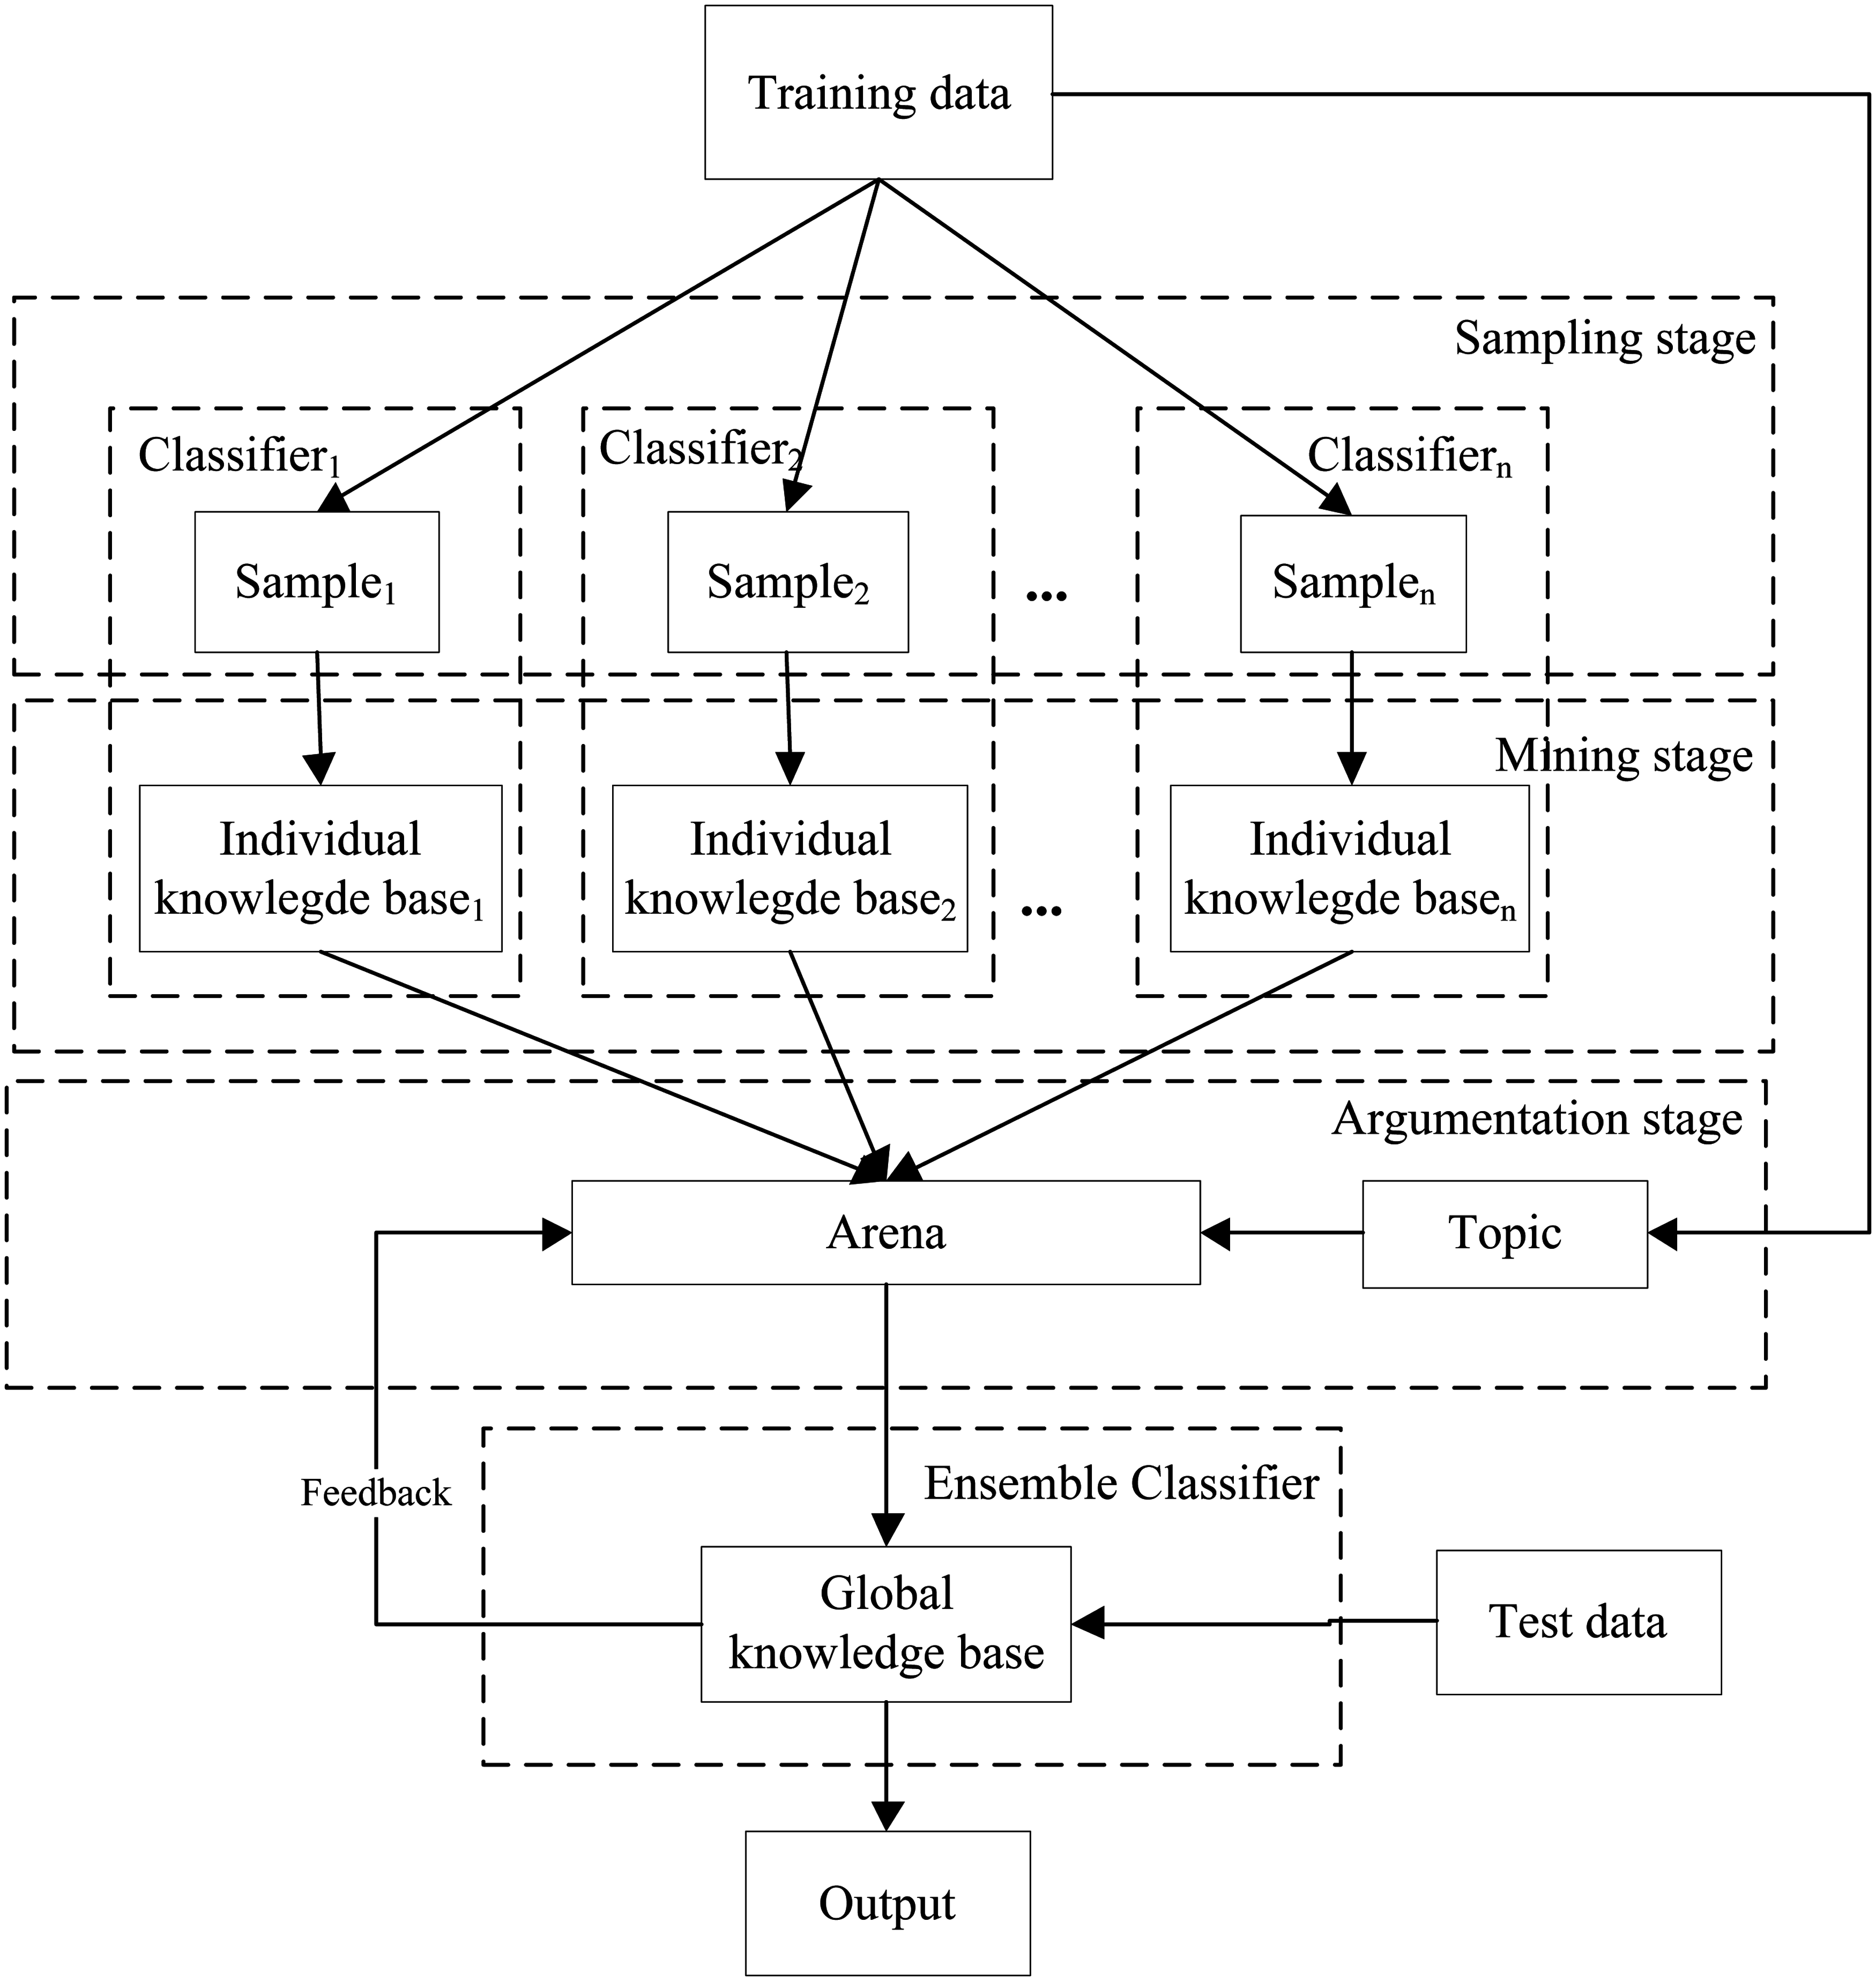
\includegraphics[width=3in]{images/ensemble.png}
  \caption{Ensemble Learning \cite{ensemblelearning}}
  \label{fig:ens}
\end{figure}
\subsection{Argumentation Interchange Format}
In order to enable true interoperability of arguments and argumentstructures we need an argument description language that can be extended beyonda particular argumentation theory, enabling us to accommodate a variety of argumentation theories and schemes. Initial implementations of such an AIF were in the form of an Argumentation Markup Language (AML), intended for use in Araucaria systems. The syntax of AML is specified in a Document Type Definition (DTD) which imposes structural constraints on the form of valid AML documents.

However, Rahwan et al. in \cite{rahwan2009argumentation} note that AMLs present two limitations:

\begin{itemize}
  \item Each particular AML is designed for use with a particular tool. This causes a tight coupling of the AML with the specifics of theory with which the argumentation system functions. This is counterintuitive to interoperability.
  \item AMLs are primarily aimed at enabling users to structure argumentsthrough diagrammatic linkage of natural language sentences. Hence, these mark-up languages are not designed to process formal logical statements such as those used within multi-agent systems.
\end{itemize}

In order to overcome the above limitations, researchers gathered to create an Argumentation Interchange Format which consolidates work in AMLs and multi agent systems  by focusing on two aims: to facilitate the development of (closed or open) multi-agent systems capable of argumentation-based reasoning and interaction using a shared formalism and to facilitate data interchange among tools for argument manipulation and argument visualization.

A modern AIF, named ArgDown, is shown in Fig \ref{argdown}. It places focus on quick visualization of given arguments written using a specific syntax.
\begin{figure}
  \centering
  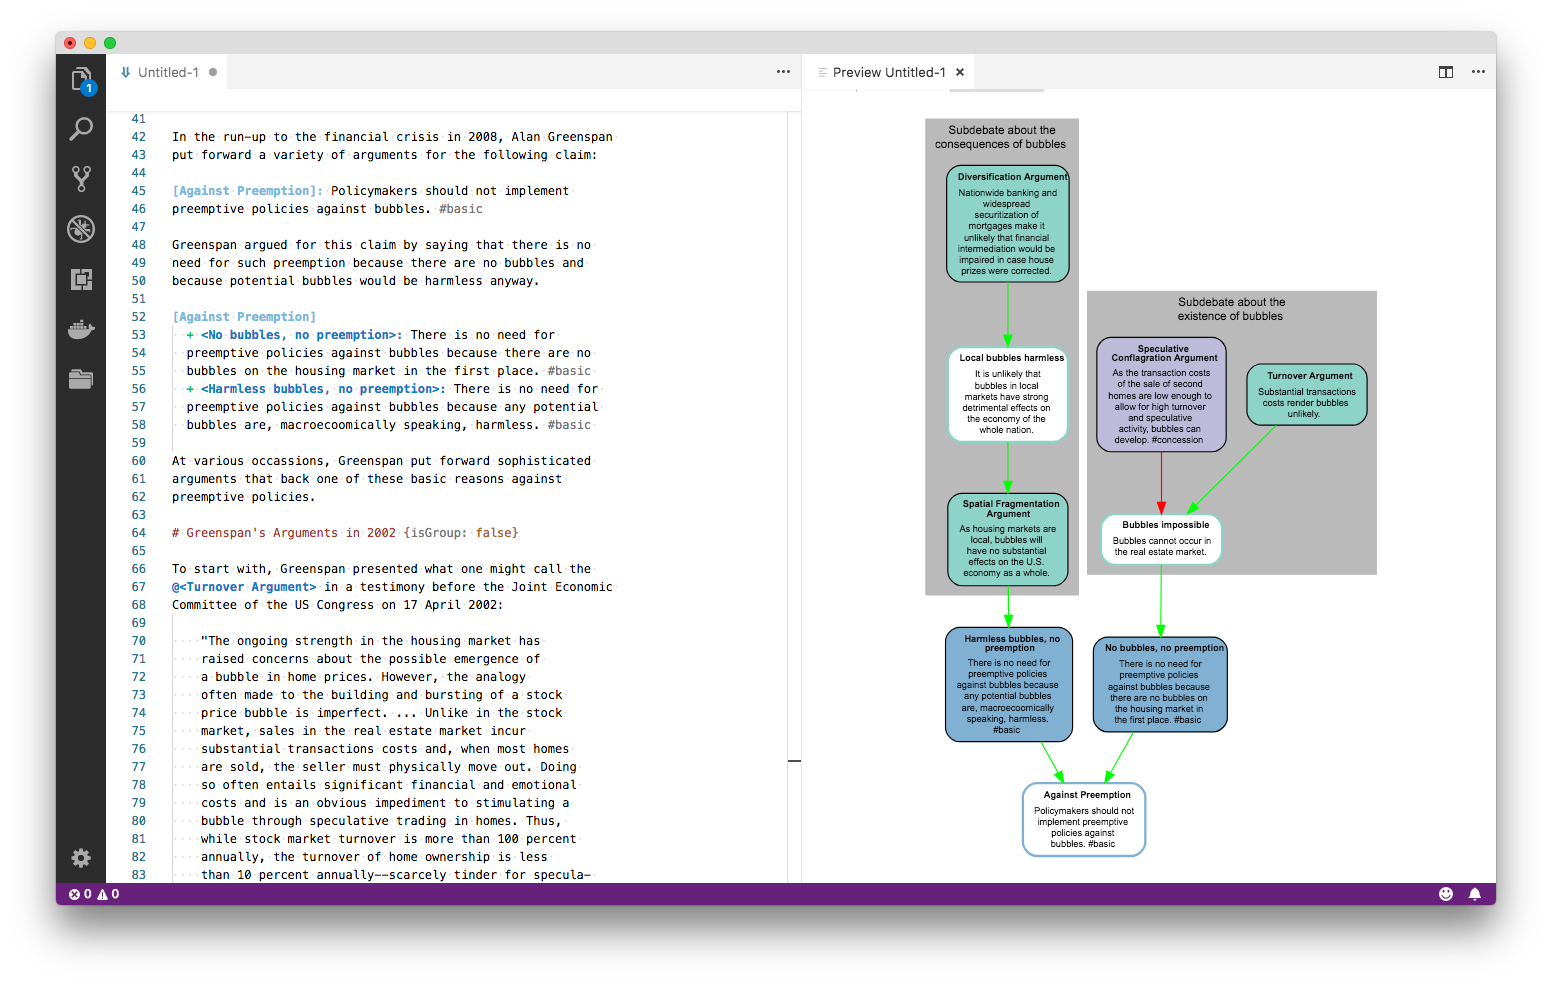
\includegraphics[width=3in]{images/argdown.png}
  \caption{ArgDown Language [https://argdown.org/]}
  \label{argdown}
\end{figure}

Rahwan et al. in \cite{rahwan2007laying} provide the groundwork for a World Wide Argument Web using AIFs. They mention the need for an WWAW to be able to store, create, update and query argumentative structures, have web accessible repositories, be based on open standard frameworks, and support the representation of arguments using a wide variety of argumentation schemes. 

\subsection{Subjective Logic in Assurance Cases}
An assurance case is a collection of auditable claims, arguments, and evidence created to support the contention that a defined system/service will satisfy the particular requirements, such as safety, reliability, or
security. Assurance cases have been used in many industries, especially in safety-critical areas. A structured assurance case
explicitly explains how the evidence supports the claim through the argument. However, both the evidence and argument are
normally imperfect because of the inevitable fallibility of humans and limitations of time and technologies.\cite{yuan2017subjective}

To measure the confidence in the assurance case, the authors of \cite{yuan2017subjective}
follow the law of total probability to define the concepts of confidence, sufficiency of argument and necessity of argument to represent the extent that they believe in the premise and argument respectively. They identify four basic argument types: one-to-one argument, alternative argument, conjunction argument and disjunction argument. For each
argument type, they define propagation rules to assess the confidence in the argument. Then, the confidence in assurance case is calculated from the bottom up.

\subsection{Subjective Logic and Climate Change Denial}
As part of an ongoing project tackling Climate Change Denial in public discourse such as forums, social media etc., Groza et al. published a paper in July 2018, experimenting with the use of Subjective Logic in Argumentation as proposed by Koster et al. in \cite{Koster2017}. The authors attempt to analyse various arguments on the issue of climate change, obtained from online debate websites. However, since they were dealing with a large amount of collective opinion, they realized the need to aggregate arguments to obtain a top-level view of people's beliefs. 

The authors observed that upon using the consesus operator for the aggregation of opinion on higher number of arguments, a consensual opinion had 
lower ignorance levels, therefore resulting in higher confidence levels on a given set of hypotheses. This operator also helps determine if 
an entire community is in support of a certain hypothesis by ranking the computed distance of opinions between two communities.

The authors claim that a low level of ignorance is the result of a large number of arguments being posted about this topic, which means there is a high level of interest for that topic. 
The ignorance level helped measure the expectancy of any given argument to be considered an \textit{accepted argument}.

Upon analysis of the clustered hypotheses, the authors note that out of 193 clusters, only one cluster had a balanced score in favour of a higher disbelief degree for the hypothesis:
 \textit{Developed countries should have a moral obligation to mitigate the effects of climate change}, as well as the lowest ignorance score. They claim that their approach for analysing people's arguments can be applied in different domains, other than the one exemplified in the paper, i.e. climate change.

\section{Conclusion}
In this essay, we described the contributions of various researchers to the implementation of argumentation theory in artificial intelligence and subjective logic in argumentation. We first defined basic concepts of argumentation theory and formalism for representation of argumentation in the form of AAFs which serve as the basis for any discussion regarding argumentation in AI. 
We also took a look at the problems faced in the application of argumentation. These problems were solved using Subjective Logic. Finally, we studied about the practical applications of subjective logic in argumentation in various fields of discourse.

The use of Subjective Logic in Argumentation and AI is a relatively new concept. While not a lot of research has been done in this particular domain, argumentation theory is a very broad field that combines philosophy, linguistics, computation, and logic, attracting researchers from all of these fields. In the past year, there has been a slight surge in research of SL implementation in argumentation. Hopefully, in the near future, there will be further theoretical research and practical applications of this field. 
% The next two lines define the bibliography style to be used, and the bibliography file.
\bibliographystyle{ACM-Reference-Format}
\bibliography{sample-base}

\end{document}
